\documentclass{article}
\usepackage{graphicx} % Required for inserting images
\usepackage{amsmath}
\usepackage{float}

\title{FIR Filter Design Report}
\author{Name: Geetesh Kini, Roll no: 210070041, Filter no: 104, Group No: 15,\\ Reviewed by Group member: Chanakya Varude, Roll no: 210070092}
\date{March 2023}

\begin{document}

\maketitle

\tableofcontents
\clearpage

\section{Filter Details (Bandpass)}

\subsection{Un-normalized Discrete Time Filter Specifications}

Filter number = 104\\
Since filter number $>$ 80, m = 104 - 80 = 24 and passband will be equiripple.\\
q(m) = greatest integer strictly less than 0.1*m = 2\\
r(m) = m - 10*q(m) = 4\\
$B_L$(m) = 10 + 5*q(m) + 13*r(m) = 10 + 5*2 + 13*4 = 72KHz \\
$B_H$(m) = $B_L$(m) + 75 = 147KHz\\

\vspace{1.5em}
\noindent

This filter is given to be a Bandpass Filter with passband from BL(m) kHz to BH(m) kHz.
Therefore the specifications are:
\begin{itemize}
    \item Passband : \textbf{72 - 147 KHz}
    \item  Transition band : \textbf{5KHz} on either side of stopband
    \item Stopband : \textbf{0 - 67} and \textbf{152 - 300 KHz} (As \textbf{sampling rate} is \textbf{600KHz})

    \item  Tolerance : \textbf{0.15} in \textbf{magnitude} for both passband and stopband
\end{itemize}

\subsection{Normalized Digital Filter Specifications}
Sampling rate = 600KHz\\
In the normalized frequency axis, sampling rate corresponds to 2$\pi$\\
Therefore, any frequency can be normalized as follows :
\begin{equation*}
    \omega = \frac{\Omega*2\pi}{\Omega_s}
\end{equation*}
where $\Omega_s$ is the Sampling Rate.\\

\vspace{1em}
\noindent
For the normalized discrete filter specifications, the nature and tolerances being the dependent variables remain the same while the passband and stopband frequencies change as per the above transformations. 
\begin{itemize}
    \item Passband : (\textbf{0.24 -  0.49}) {$\pi$}
    \item  Transition band : \textbf{0.017} $\pi$ on either side of stopband
    \item Stopband : (\textbf{0 - 0.223}) {$\pi$} and (\textbf{0.507 - 1}) {$\pi$}
    \item  Tolerance : \textbf{0.15} in \textbf{magnitude} for both passband and stopband
\end{itemize}

\subsection{FIR Filter Transfer Function using Kaiser Window}

The tolerance in both the stopband and passband is given to be 0.15.\\
Therefore $\delta$ = 0.15 and we get the minimum stopband attenuation to be:-

\begin{center}
    A = -20 log(0.15) = 16.4782dB
\end{center}

Since A < 21, we get $\beta$ to be 0 where $\beta$ is the shape parameter of Kaiser window.\\
Now to estimate the window length required, we use the empirical formula for the lower bound on
the window length.

\begin{center}
    \begin{equation*}
        N \geq \frac{A-8}{2.285*\Delta w_T}
    \end{equation*}
\end{center}

Here $\Delta w_T$ is the minimum transition width. In our case, the transition width is the same on either
side of the passband.

\begin{center}
    \begin{equation*}
        \Delta w_T = \frac{5KHz*2\pi}{600KHz} = 0.017 \pi
    \end{equation*}
\end{center}

\begin{center}
    Hence, N $\geq$ 71
\end{center}

The above equation gives a loose bound on the window length when the tolerance is not very stringent. On successive trials in MATLAB,it was found that a window length of $\textbf{99}$ is required to satisfy
the required constraints. Also, since $\beta$ is 0, the window is actually a rectangular window.
\newline

The time domain coefficients were obtained by first generating the ideal impulse response samples
for the same length as that of the window. The Kaiser Window was generated using the MATLAB
function and applied on the ideal impulse response samples. For generating the ideal impulse response a separate function was made to generate the impulse response of Low-Pass filter. It took the
cutoff value and the number of samples as input argument. The band-pass impulse response samples
were generated as the difference between two low-pass filters as done in class.\\

The impulse response sequence that we get from MATLAB is: (Note that the values are from n = -49 to 49)

\begin{verbatim}
 Columns 1 through 9

-0.0121   -0.0008    0.0089    0.0044    0.0000    0.0058   0.0064   -0.0073   -0.0153

  Columns 10 through 18

-0.0042    0.0071    0.0031   -0.0001    0.0095    0.0120   -0.0052   -0.0181   -0.0079    

  Columns 19 through 27

0.0046   -0.0001   -0.0024    0.0131    0.0202   -0.0008    -0.0203   -0.0113    0.0018

  Columns 28 through 36

-0.0061   -0.0089    0.0162    0.0326    0.0073   -0.0222   -0.0141   -0.0000   -0.0175

  Columns 37 through 45

-0.0254    0.0186    0.0575    0.0250   -0.0260   -0.0160    0.0033   -0.0516    -0.0940

  Columns 46 through 54

0.0198    0.1929    0.1564   -0.1065   -0.2666   -0.1065    0.1564    0.1929    0.0198

  Columns 55 through 63

-0.0940   -0.0516    0.0033   -0.0160   -0.0260    0.0250    0.0575    0.0186   -0.0254

  Columns 64 through 72

-0.0175   -0.0000   -0.0141   -0.0222    0.0073    0.0326    0.0162   -0.0089   -0.0061

  Columns 73 through 81

0.0018   -0.0113   -0.0203   -0.0008    0.0202    0.0131    -0.0024   -0.0001    0.0046

  Columns 82 through 90

-0.0079   -0.0181   -0.0052    0.0120    0.0095   -0.0001    0.0031    0.0071   -0.0042

  Columns 91 through 99

-0.0153   -0.0073    0.0064    0.0058    0.0000    0.0044    0.0089   -0.0008   -0.0121
\end{verbatim}

\vspace{5mm}

The z-transform can simply be read off from the sequence values since its finite sequence.
\clearpage

\section{Filter Details (Bandstop)}
\subsection{Un-normalized Discrete Time Filter Specifications}

Filter number = 104\\
Since filter number $>$ 80, m = 104 - 80 = 24 and passband will be monotonic.\\
q(m) = greatest integer strictly less than 0.1*m = 2\\
r(m) = m - 10*q(m) = 4\\
$B_L$(m) = 20 + 3*q(m) + 11*r(m) = 20 + 3*2 + 11*4 = 70KHz \\
$B_H$(m) = $B_L$(m) + 40 = 110KHz\\

\vspace{1.5em}
\noindent

This filter is given to be a Bandstop Filter with stopband from BL(m) kHz to BH(m) kHz.
Therefore the specifications are:
\begin{itemize}
    \item Stopband : \textbf{70 - 110 KHz}
    \item  Transition band : \textbf{5KHz} on either side of stopband
    \item Passband : \textbf{0 - 65} and \textbf{115 - 212.5 KHz} (As \textbf{sampling rate} is \textbf{425KHz})

    \item  Tolerance : \textbf{0.15} in \textbf{magnitude} for both passband and stopband
\end{itemize}


\subsection{Normalized Digital Filter Specifications}
Sampling rate = 425KHz\\
In the normalized frequency axis, sampling rate corresponds to 2$\pi$\\
Therefore, any frequency can be normalized as follows :
\begin{equation*}
    \omega = \frac{\Omega*2\pi}{\Omega_s}
\end{equation*}
where $\Omega_s$ is the Sampling Rate.\\

\vspace{1em}
\noindent
For the normalized discrete filter specifications, the nature and tolerances being the dependent variables remain the same while the passband and stopband frequencies change as per the above transformations. 
\begin{itemize}
    \item Stopband : (\textbf{0.329 -  0.518}) {$\pi$}
    \item  Transition band : \textbf{0.024} $\pi$ on either side of stopband
    \item Passband : (\textbf{0 - 0.306}) {$\pi$} and (\textbf{0.541 - 1}) {$\pi$}
    \item  Tolerance : \textbf{0.15} in \textbf{magnitude} for both passband and stopband
\end{itemize}

\subsection{FIR Filter Transfer Function using Kaiser Window}

The tolerance in both the stopband and passband is given to be 0.15.\\
Therefore $\delta$ = 0.15 and we get the minimum stopband attenuation to be:-

\begin{center}
    A = -20 log(0.15) = 16.4782dB
\end{center}

Since A < 21, we get $\beta$ to be 0 where $\beta$ is the shape parameter of Kaiser window.\\
Now to estimate the window length required, we use the empirical formula for the lower bound on
the window length.

\begin{center}
    \begin{equation*}
        N \geq \frac{A-8}{2.285*\Delta w_T}
    \end{equation*}
\end{center}

Here $\Delta w_T$ is the minimum transition width. In our case, the transition width is the same on either
side of the stopband.

\begin{center}
    \begin{equation*}
        \Delta w_T = \frac{5KHz*2\pi}{425KHz} = 0.024 \pi
    \end{equation*}
\end{center}

\begin{center}
    Hence, N $\geq$ 51
\end{center}

The above equation gives a loose bound on the window length when the tolerance is not very stringent. On successive trials in MATLAB,it was found that a window length of $\textbf{77}$ is required to satisfy
the required constraints. Also, since $\beta$ is 0, the window is actually a rectangular window.
\newline

The time domain coefficients were obtained by first generating the ideal impulse response samples
for the same length as that of the window. The Kaiser Window was generated using the MATLAB
function and applied on the ideal impulse response samples. For generating the ideal impulse response a separate function was made to generate the impulse response of Low-Pass filter. It took the
cutoff value and the number of samples as input argument.The bandstop impulse response samples
were generated as the difference between three low-pass filters( all-pass - bandpass ) as done in class.\\

The impulse response sequence that we get from MATLAB is: (Note that the values are from n = -38 to 38)

\begin{verbatim}
    Columns 1 through 9

-0.0014    0.0021   -0.0069   -0.0122    0.0055    0.0192    0.0031   -0.0148   -0.0068

  Columns 9 through 18

0.0032   -0.0021   0.0020    0.0170    0.0062   -0.0229   -0.0186    0.0136    0.0187

  Columns 19 through 27

-0.0011   -0.0015    0.0038   -0.0177   -0.0248    0.0182    0.0443    0.0008   -0.0387

  Columns 28 through 36

-0.0138    0.0088   -0.0085    0.0126    0.0655    0.0124   -0.1182   -0.0885    0.1178

  Columns 37 through 45

0.1744   -0.0495    0.7880   -0.0495    0.1744    0.1178   -0.0885   -0.1182    0.0124

  Columns 46 through 54

0.0655    0.0126   -0.0085    0.0088   -0.0138   -0.0387    0.0008    0.0443    0.0182

  Columns 55 through 63

-0.0248    -0.0177    0.0038   -0.0015   -0.0011    0.0187    0.0136   -0.0186   -0.0229

  Columns 63 through 72

0.0062    0.0170    0.0020    -0.0021    0.0032   -0.0068   -0.0148    0.0031    0.0192

  Columns 72 through 77

0.0055   -0.0122   -0.0069    0.0021   -0.0014

\end{verbatim}

\vspace{5mm}

The z-transform can simply be read off from the sequence values since its finite sequence.
\clearpage

\section{Matlab Plots}

\subsection{BandPass Filter}

\begin{figure}[h!]

\centering
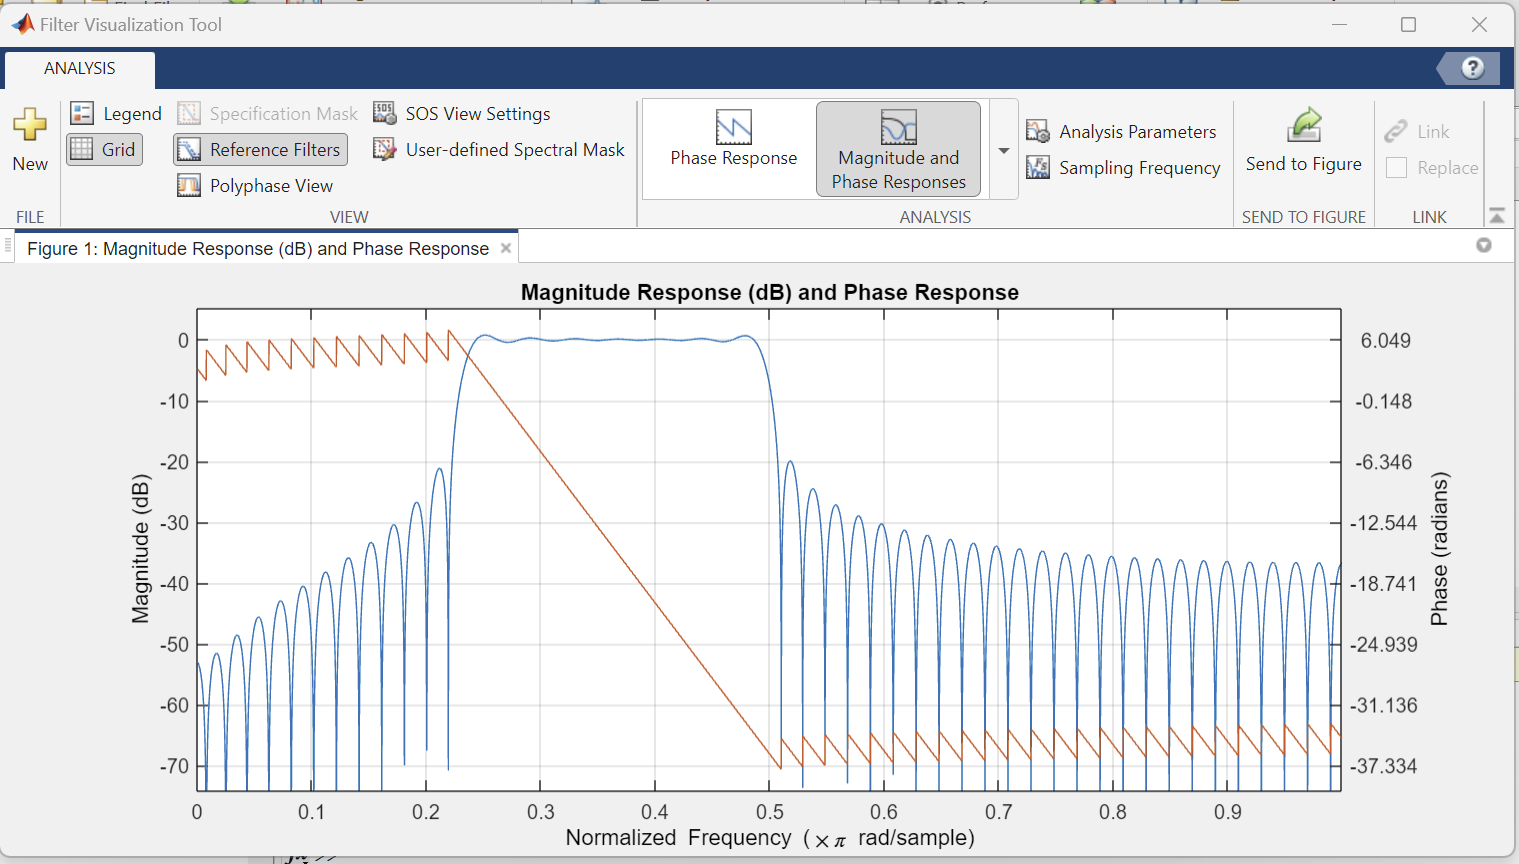
\includegraphics[scale = 0.6]{Bode.png}
\caption{Frequency Response}
\end{figure}

It can be seen that the FIR Filter is indeed giving us a Linear Phase response which is
desired.

\clearpage

\begin{figure}[h!]

\centering
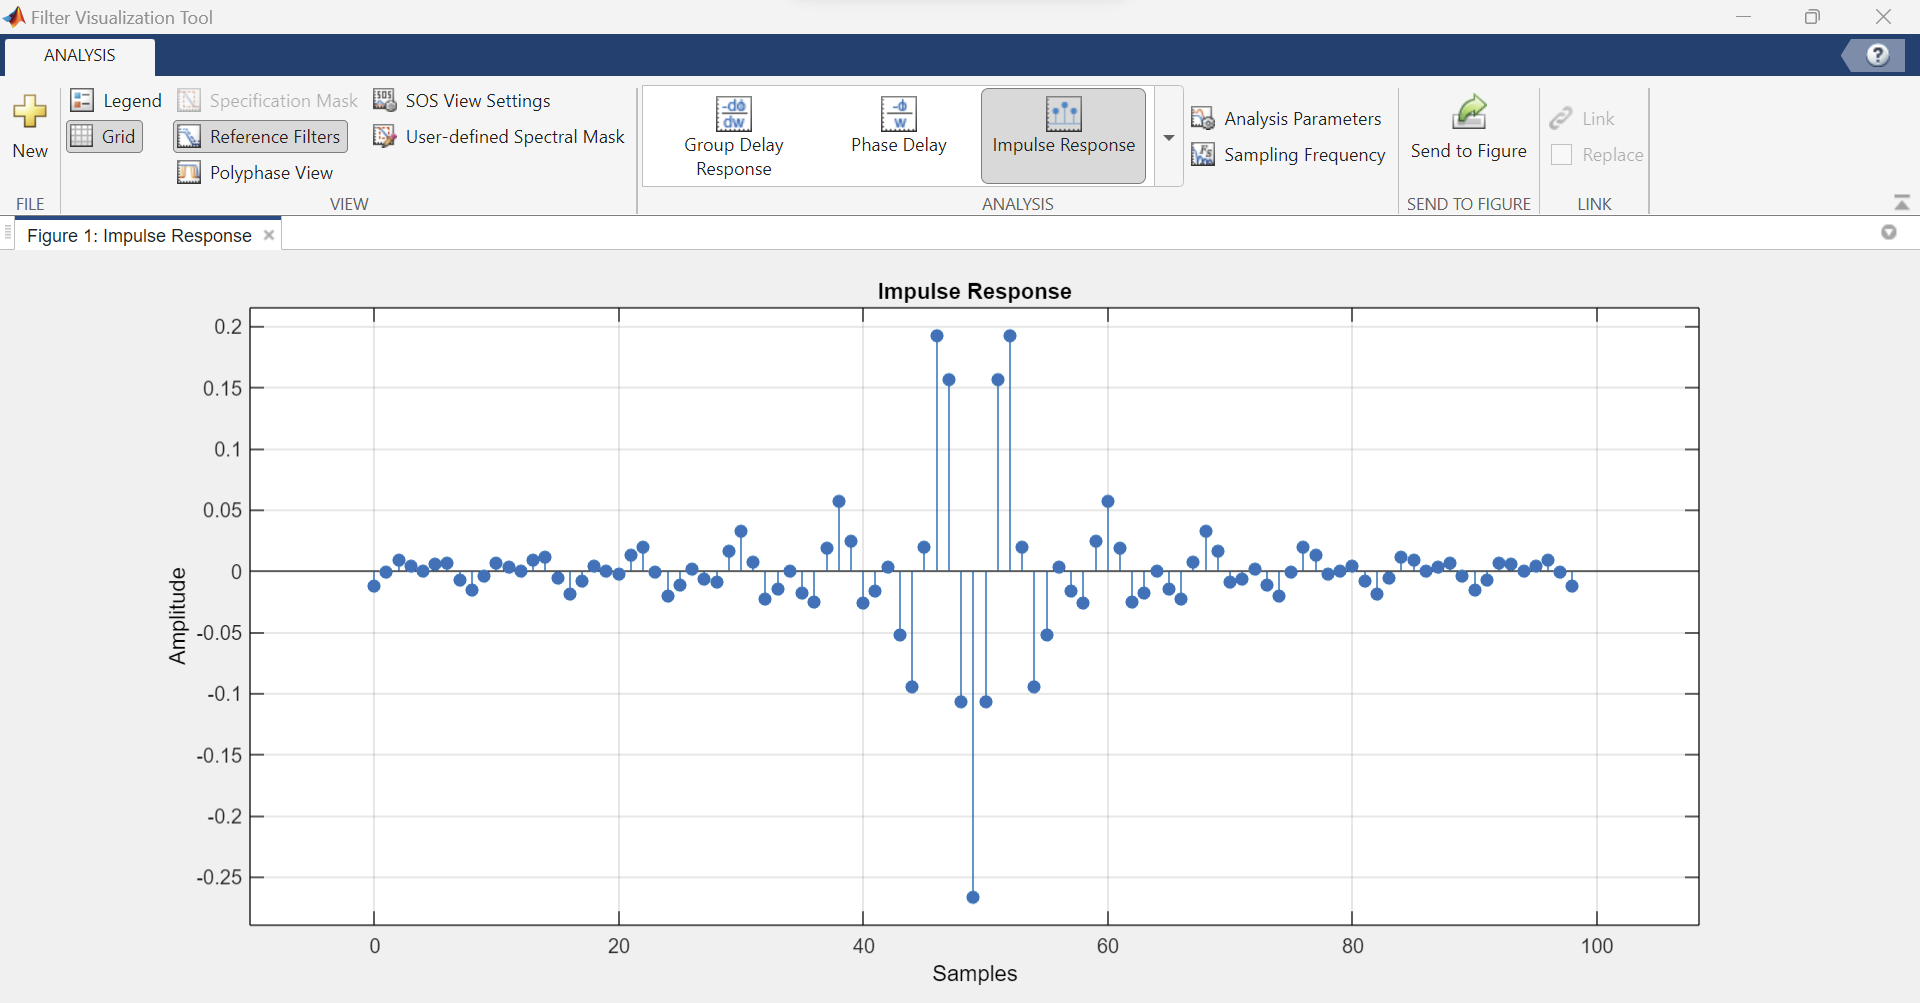
\includegraphics[scale = 0.45]{Impulse res.png}
\caption{Impulse Response}
\end{figure}

\begin{figure}[h!]

\centering
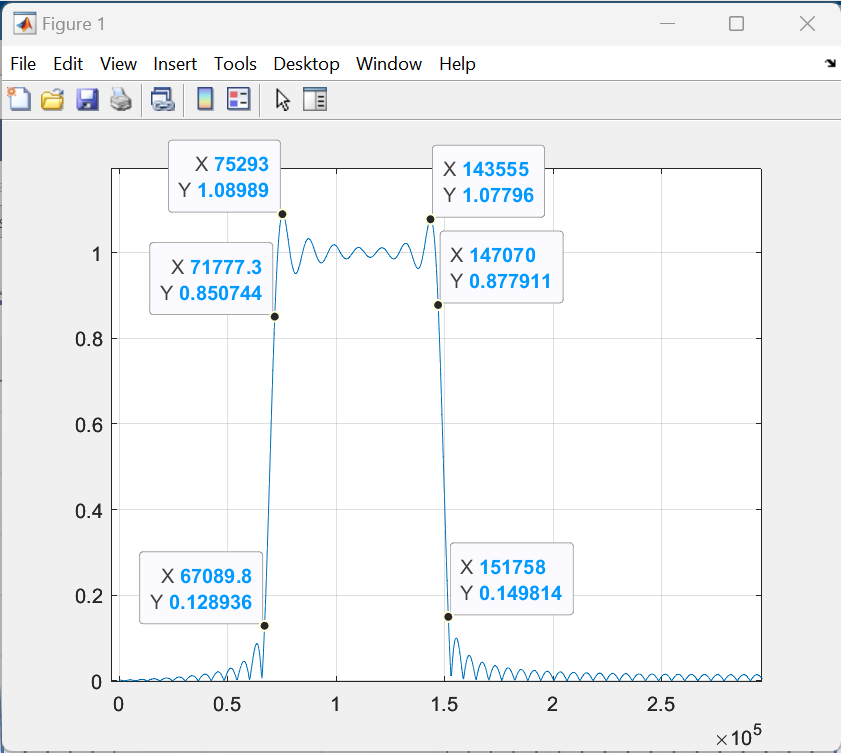
\includegraphics[scale = 0.58]{Freq Res.png}
\caption{Magnitude plot}
\end{figure}

From the above figure, it can be seen that all the specifications have been satisfied.

\subsection{BandStop Filter}

\begin{figure}[h!]

\centering
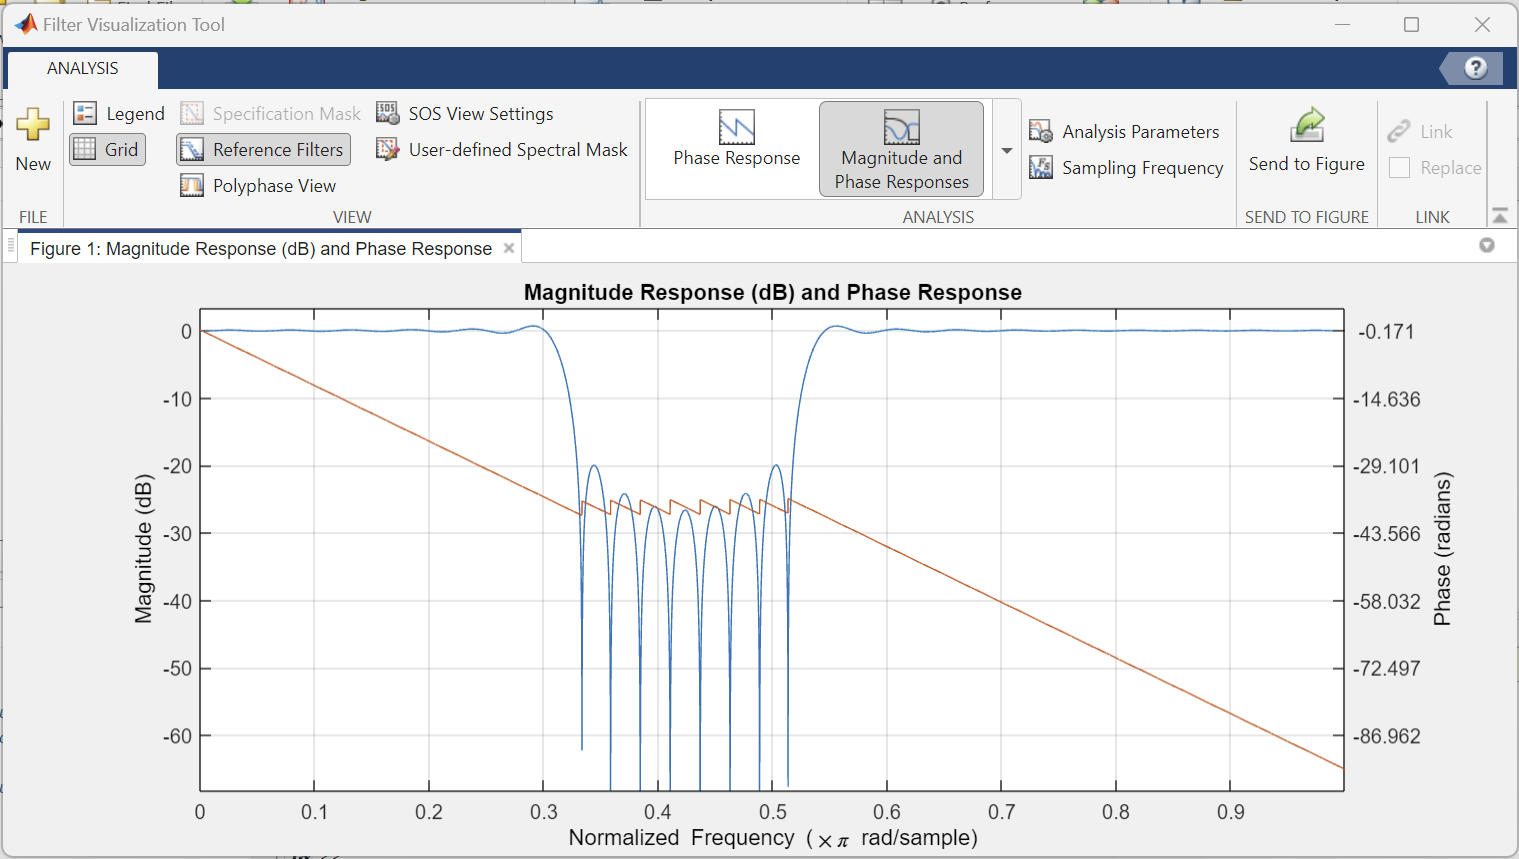
\includegraphics[scale = 0.6]{Bandstop_Mag.png}
\caption{Frequency Response}
\end{figure}

It can be seen that the FIR Filter is indeed giving us a Linear Phase response which is
desired.

\clearpage

\begin{figure}[h!]

\centering
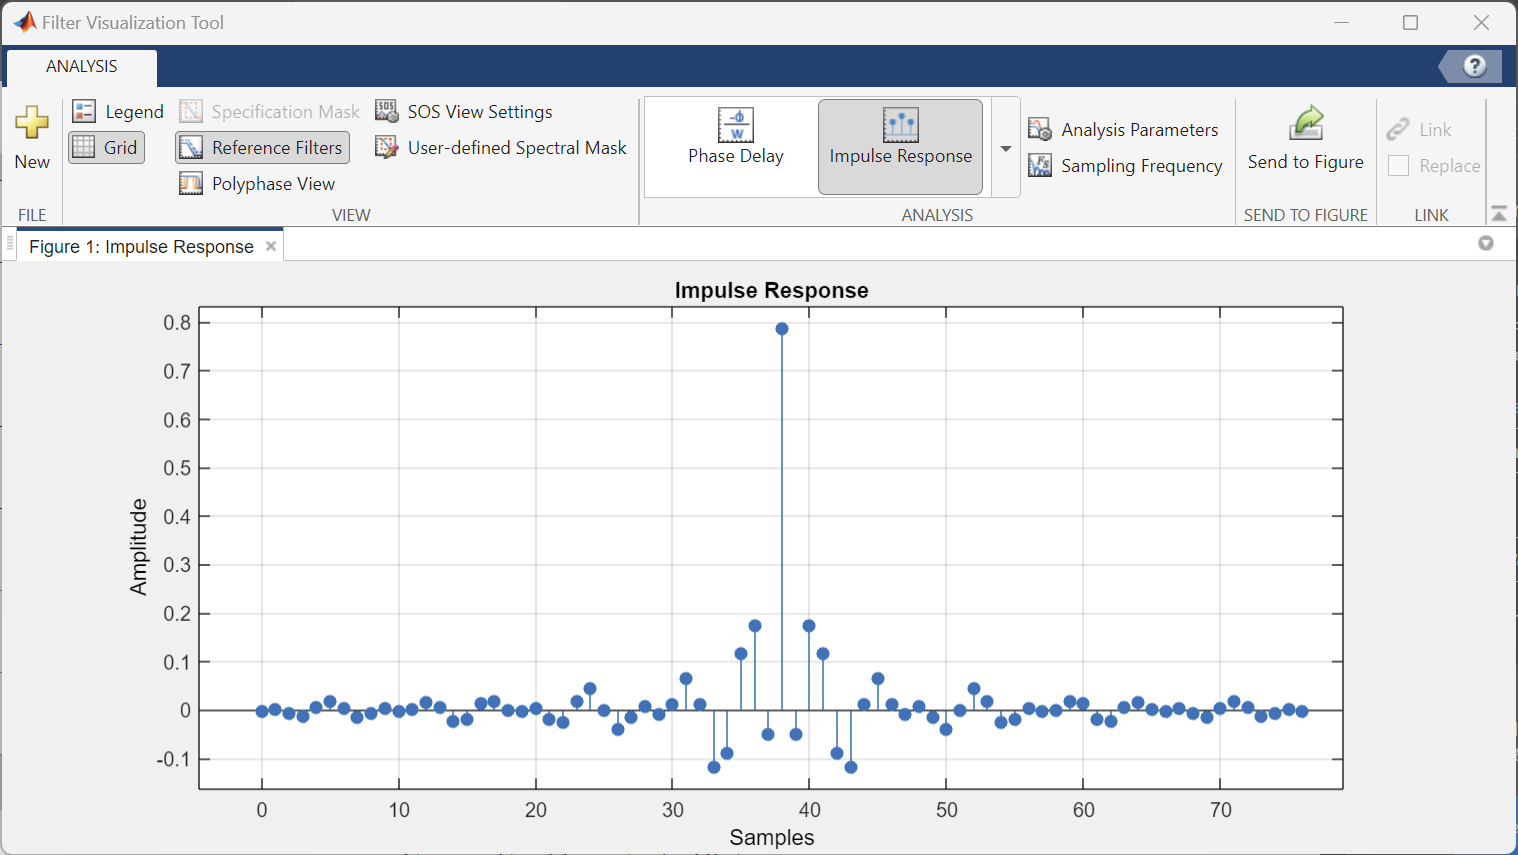
\includegraphics[scale = 0.45]{Impulse Response_Bandstop.png}
\caption{Impulse Response}
\end{figure}

\begin{figure}[h!]

\centering
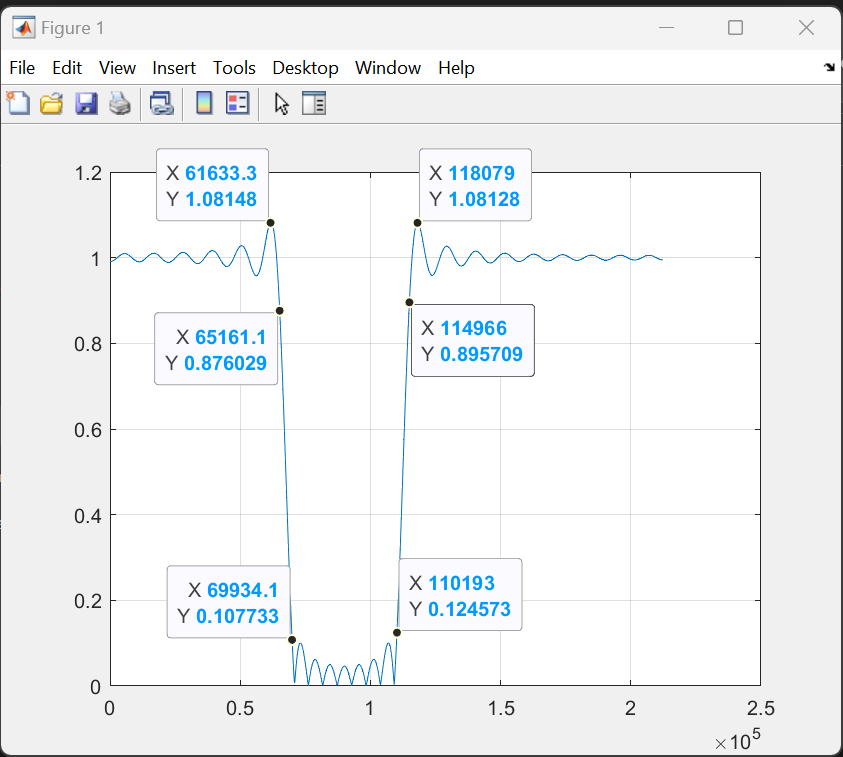
\includegraphics[scale = 0.58]{Bandstop_Freq.png}
\caption{Magnitude plot}
\end{figure}

From the above figure, it can be seen that all the specifications have been satisfied.

\clearpage

\section{Comparison Between FIR and IIR Realizations}

Advantages of FIR Filters over IIR filters:
\begin{itemize}
    \item We get a linear phase response in FIR filters, which we don't get using IIR filters.
    \item The effort required to implement FIR Filters is also easier as we have to just truncate the ideal impulse response using the window function, whereas for IIR, we need to find the analog filter specs, then design low pass filter, and then convert it into the required filter.
\end{itemize}

Advantages of IIR Filters over FIR filters:
\begin{itemize}
    \item We don't have any control over the nature of passband and stopband in FIR filters, whereas in IIR filters, we can control that.
    \item We can't control the tolerances of passband and stopband independently in FIR filters. In IIR filters, we can do that.
    \item The Passband for IIR filters is more specific as it keeps the value of transfer function always less than 1, but in FIR, the value of transfer function can be more than, or less than 1.
    \item We usually need a lot more resources for FIR filters as compared to IIR filters, as we can see that the value of N for FIR filters is considerably large.
\end{itemize}

So, each type of filter has its own advantage, we can choose the one we want according to our needs.

\section{Peer Review of Assignment}

I have reviewed the report of my peer:

\begin{center}
    Annirudh K P\\
    (Roll no: 210070009, Filter number: 96)
\end{center}
and certify it to be correct.

\end{document}
